\documentclass{beamer}
%\usetheme{Antibes}
%\usetheme{Dresden}
\usetheme{Frankfurt}
%\usetheme{Copenhagen}
%\usetheme{Darmstadt}
%\usecolortheme{dolphin}
\usepackage{cancel}
\usepackage{tikz}
%%%%%%%%%%%%%%%%%%%%%%%%%%%%%%%%%%%%%%%%%%%%%%%%%%%%%%%%
\usepackage{multicol}

\newtheorem{proposition}[theorem]{Proposition}
\newtheorem{remark}[theorem]{Remark}
\newtheorem*{remark*}{Remark}
\newtheorem{conjecture}[theorem]{Conjecture}
\newtheorem{claim}[theorem]{Claim}
\newtheorem*{claim*}{Claim}
\usepackage{xcolor}
\usepackage{longtable}
\usepackage{hyperref}
\newtheorem{openproblem}[theorem]{Open Problem}


\setbeamertemplate{blocks}[rounded][shadow=true]

\setbeamertemplate{theorems}[ams style]
\begin{document}
	\title[]{\textcolor{black}{\textbf{Linear Regression Analysis for the Kings County's (Seattle, WA) House Market.}}}
	
	\author[Yevgeniy Kostrov \hspace{1in} kostrovy@mville.edu]
	{\textcolor{black}
	{\textbf{by Y.~Kostrov\inst}}}
	\date[April 14, 2019]

%
%	Title Page:
%	

%	{
%\usebackgroundtemplate{\includegraphics[height=\paperheight,width=\paperwidth]{london}}
%\frame{
%}
%}
	\begin{frame}	
			\maketitle
	\end{frame}
\begin{frame}{\contentsname}
	\begin{multicols}{2}
		\tableofcontents
	\end{multicols}
\end{frame}
%
%
%	
%
%
%}
\section{Overview}
\frame{
\frametitle{Overview }
\begin{center}
	The purpose of this project is to analyze a data set containing data about houses sold in Kings County (Seattle, WA).
\end{center}
}
\frame{
	\frametitle{Overview }
During the analysis:
\pause
\begin{enumerate}
	\item I will perform necessary data wrangling first.
	\pause
	\item I will build a Linear Regression Model with one explanatory variable.:
	\pause
		\begin{itemize}
			\item I will check statistical assumptions for the linear regression model
			\item I will explain the model, including intercept, coefficient for the explanatory variable, $R^2$, and ANOVA
		\end{itemize}
	\pause
	\item I will build a Multiple Linear Regression Model with many explanatory variables.
	\pause
	\begin{itemize}
		\item I will check statistical assumptions for the multiple linear regression model
		\item I will explain the model, including intercept, coefficients for the explanatory variables, $R^2$, and ANOVA
	\end{itemize}
\end{enumerate}
}
\section{Business Problem}
\frame{
\frametitle{Business Problem}
\begin{itemize}
	\item The fair price of the house is a hard quantity to assess. 
	\vskip 0.3in
	\pause
	\item Both sellers and buyers would like to know the best price for the house. 
	\vskip 0.3in
	\pause
	\item Which features of the property would be the best predictors of the value? 
	\vskip 0.3in
	\pause
	\item I will build a regression model that helps  predict the value of the house.
	\vskip 0.3in
	\pause
	\item  I will, also, check the necessary statistical assumptions for the regression model and explain the model's parameters.
\end{itemize}
}
\section{Data Description}
\frame{
\frametitle{Data Description}
\begin{itemize}
	\item The file called ``kc\_house\_data.csv''  in the data  folder of the project holds the data for this project.
	\vskip 0.3in
	\pause
	\item This project will use this data about Kings County's(Seattle, WA) housing market to create Linear Regression Model.
	\vskip 0.3in
	\pause
	\item The data file contains numerous columns with information about properties sold such as price, size of the  living area, size of the basement, number of bedrooms, etc.
\end{itemize}
}
\section{My Python Package}
\frame{
\frametitle{My Python Package}
\begin{itemize}
	\item While working on this project, I have created my own Python package with helping functions.
	\vskip 0.2in
	\pause
	\item The most important function in this package is ``evaluate\_model.py''(in the ``src'' folder). This function:
	\vskip 0.2in
	\pause
	\begin{itemize}
		\item  creates the model from the data frame.
		\vskip 0.1in
		\pause
		\item prints out the model summary of Linear Regression.
		\vskip 0.1in
		\pause
		\item performs the checks for the statistical  assumptions of the Linear Regression.
		\vskip 0.1in
		\pause
		\item performs  a lot of different visualizations.
	\end{itemize}
\end{itemize}
}
\section{Modeling}
\frame{
	\frametitle{Modeling}
	\begin{itemize}
		\item 	My first goal was to create linear regression model with one independent variable.
		\vskip 0.1in
		\pause
		\item 	I created the correlation matrix and heat map for visualization purpose.
		\pause
		\begin{center}
			\resizebox{0.6\textwidth}{!}{
				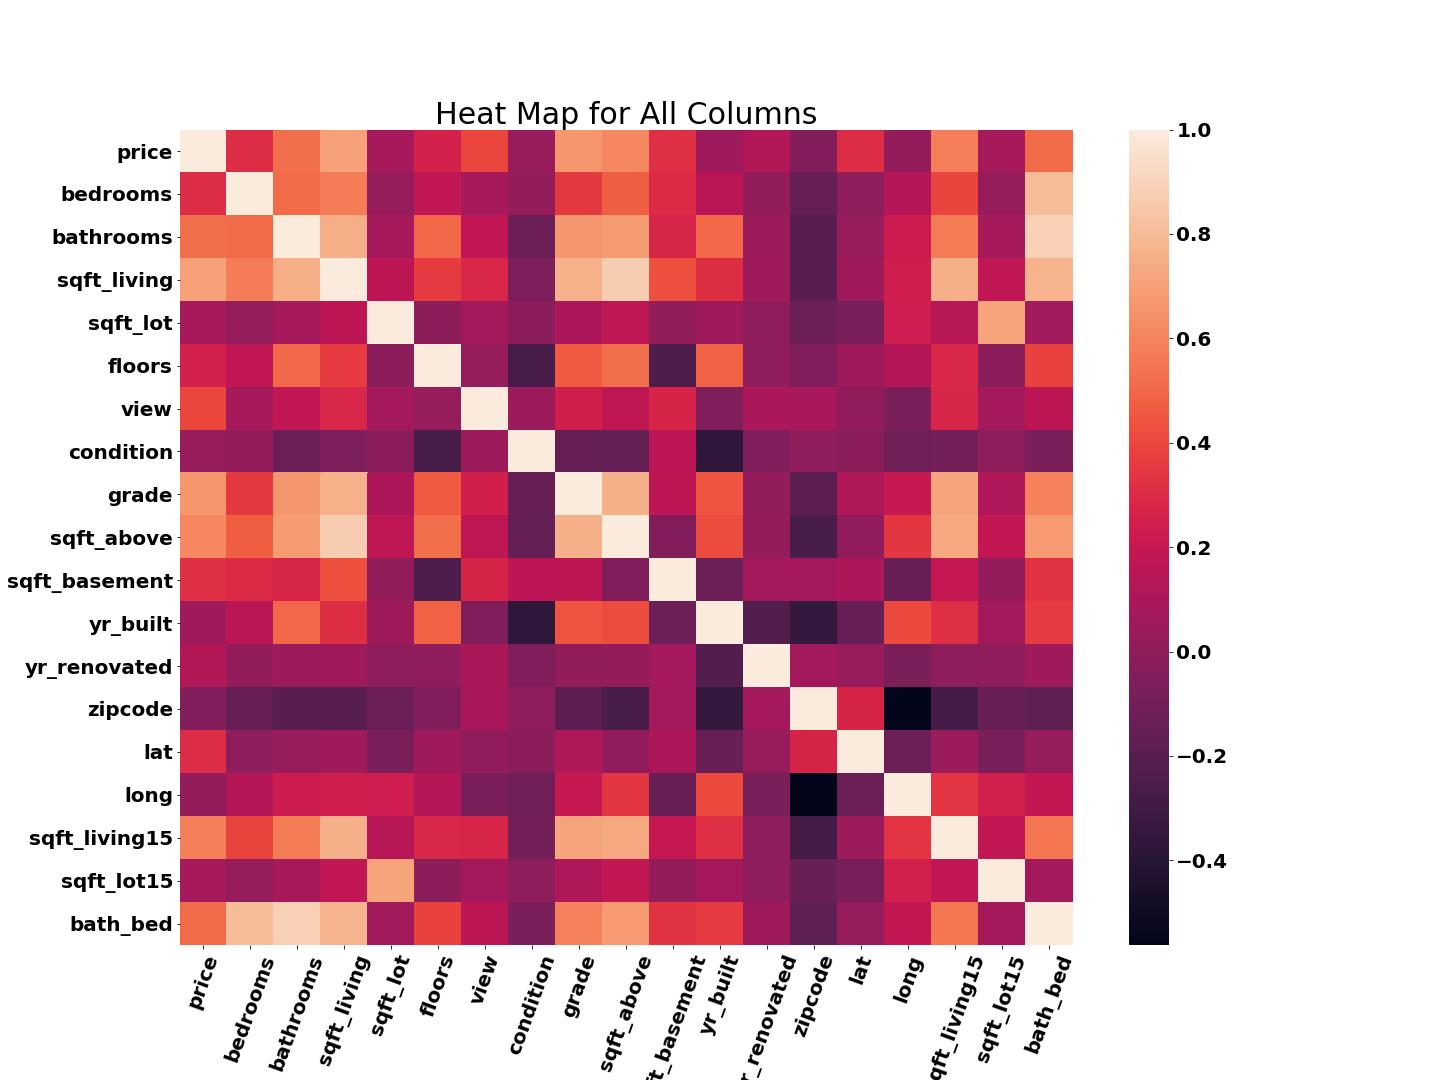
\includegraphics{heat_map.png}\label{heatmap}
			}
		\end{center}
	\end{itemize}
}
\section{Linear Model}
\subsection{Building the Linear Model}
\frame{
\frametitle{Selection of the explanatory variable for the Linear Model}
\begin{itemize}
	\item  ``sqft\_living'' has the highest correlation of  \(0.71\) with the ``price''. 
	\vskip 0.3in
	\pause
	\item  I build a regression model for the ``price'' to be predicted by ``sqft\_living''.
	\vskip 0.3in
	\pause 
	\item The model is \( \ln\left(\text{\it price}\right)  = 11.9524 + 0.0029 \cdot \text{\it sqft\_living}^{0.78}  \)
\end{itemize}
}
\subsection{Checking Statistical Hypotheses}
\frame{
\frametitle{Checking Statistical Hypotheses: Linearity}
\small
\textbf{The Null Hypothesis:}\\  The model is linearly predicted by the feature,\\
\vskip 0.1in
\pause
\textbf{The Alternative Hypothesis:\\}  The model is not linearly predicted by the feature.\\
\pause
\vskip 0.2in
\begin{itemize}
	\item Our p-value for this model is \(p=0.877 > 0.05 = \alpha\). 
	\item We don't have enough evidence to reject \textbf{The Null Hypothesis}
	 \item We conclude that our model satisfies Linearity Assumption.
\end{itemize}
}
\frame{
\frametitle{Checking Statistical Hypotheses: Normality 1}

To check Normality, I used the following checks:\\
	\begin{center}
		\textbf{QQ-Plot}\\
		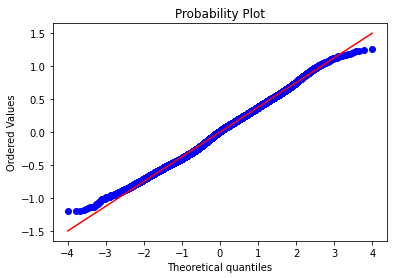
\includegraphics[width=2in,height=2in]{qq_plot_linear_model}
	\end{center}%
}

\frame{
	\frametitle{Checking Statistical Hypotheses: Normality 2}
	\begin{center}
		\textbf{DISTRIBUTIONS PLOT OF RESIDUALS}\\
		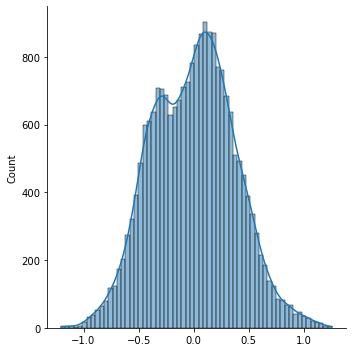
\includegraphics[width=2in,height=2in]{dist_plot_resid_linear_model}
	\end{center}%
}
\frame{
	\frametitle{Checking Statistical Hypotheses: Normality 3}
I,  also, used D'Agostino Test for Normality:\\
\vskip 0.2in 
\pause
\textbf{The Null Hypothesis:} \\ The Residuals are normally distributed
\vskip 0.1in
\pause
\textbf{The Alternative Hypothesis:} \\ The Residuals are not normally distributed.
\vskip 0.2in
\pause
\begin{itemize}
	\item Our p-value for this model is \(p=0.000 < 0.05 = \alpha\). 
	\item We have enough evidence to reject the Null Hypothesis 
	\item We conclude that D'Agostino Test tells us, that residuals are not normally distributed.
\end{itemize}
}
\frame{
\frametitle{Checking Statistical Hypotheses: Normality 3}
\textbf{Conclusion for Normality:}\\
\begin{itemize}
	\item  Based on QQ-Plot, Distributions Plot, and D'Agostino Test, I conclude that the Distribution of Errors is not far away from Normal.
	\pause 
	\vskip 0.3in
	\item  Also, since we have a lot of observations Normality Assumption doesn't play a critical role, since Central Limit Theorem will apply in this case.
\end{itemize}
}
\frame{
\frametitle{Constant Error Variance 1}
To check if heteroscedasticity is present in the model,
\begin{itemize}
	\item  I will use Residual-vs-Predicted values plot and Breusch-Pagan test.
	\item I look at at the Residual-vs-Predicted values plot first.
	\begin{center}
		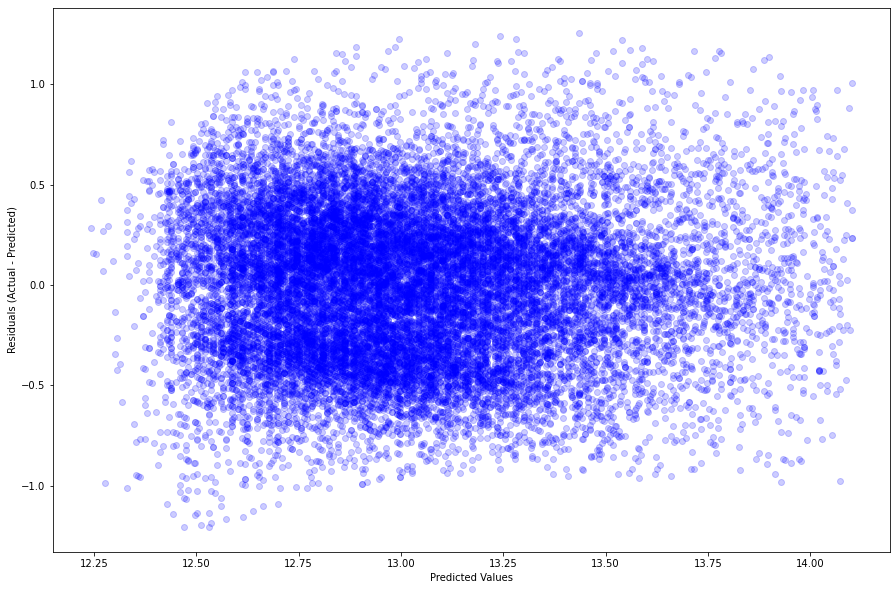
\includegraphics[width=3in]{residual_plot_linear_model}
	\end{center}
\end{itemize}
}
\frame{
\frametitle{Constant Error Variance 2}
I will use Breusch-Pagan Test:
\vskip 0.2in
\pause
\textbf{The Null Hypothesis:}\\
  Homoscedasticity is present.\\
  \textbf{The Alternative Hypothesis:}\\
  \vskip 0.1in
  \pause
  Homoscedasticity is not present (i.e. heteroscedasticity exists).\\
  \begin{itemize}
  	\item Our p-value for this model is \(p=0.12609 \ge 0.05 = \alpha\).
  	\item Thus, we don't have enough evidence to reject the Null Hypothesis and 
  	\item We conclude from Breusch-Pagan Test  , that we have don't have heteroscedasticity.
  \end{itemize}
}
\frame{
	\frametitle{Constant Error Variance 3}
\textbf{Conclusion:} \\
From the Residual-vs-Predicted values plot and  Breusch-Pagan Test, I conclude that we don't have Heteroscedasticity in our model.
}
\frame{
\frametitle{Overall Conclusion:}
\begin{center}
	\textbf{I conclude that our model satisfies statistical assumptions for the regression model.}
\end{center}
}
\subsection{Explanation of the Model}
\frame{
\frametitle{Intercept and slope 1}
Our model is 
\[ \ln\left(\text{\it price}\right)  = 11.9524 + 0.0029 \cdot \text{\it sqft\_living}^{0.78}  \]
\vspace{-0.2in}
\begin{itemize}
	\item The model has the sample intercept of \(11.9524\) and the slope of \(0.0029\).  
	\item To interpret the slope, we have to transform \(\hat{x}\) and \(\hat{y}\) towards original {\it sqft\_living} and {\it price}. 
	\item Let \(x\) = {\it sqft\_living}  and \(y\) = {\it price} for the derivation. 
	\item We have  \(\hat{x} = x^{0.78}\) and \(\hat{y} = \ln (y)\implies y  = e^{\hat{y}}\). 
\end{itemize}
}
\frame{
	\frametitle{Intercept and slope 2}
Suppose the original sqft\_living is \(x_1\) and it moved up to \(x_2\), then we have the following :
\begin{align*}
	y_1 =& e^{\hat{y}_1 }= e^{11.9524+0.0029\cdot x_1^{0.78}}  = e^{11.9524}\cdot e^{0.0029\cdot x_1^{0.78}}\\
	y_2 =& e^{\hat{y}_2 }= e^{11.9524+0.0029\cdot x_2^{0.78}}  = e^{11.9524}\cdot e^{0.0029\cdot x_2^{0.78}}
\end{align*}
\pause
To understand the change in {\it price} in percents we will use the following formula:

\begin{align*}
	100 \times \left[\frac{y_2-y_1}{y_1} \right] =& 100 \times \left[\frac{y_2}{y_1} - 1\right] = 100\times \left[\frac{ \cancel{e^{11.9524}}\cdot e^{0.0029\cdot x_2^{0.78}}}{\cancel{e^{11.9524}}\cdot e^{0.0029\cdot x_1^{0.78}}} -1 \right] \\
	=& 100 \times \left[ e^{0.0029\left( x_2^{0.78} - x_1^{0.78} \right)} -1 \right]
\end{align*}
}
\frame{
	\frametitle{Example}
For example, if the {\it sqft\_living} is \(1000ft\) and we increase it to \(1100ft\), we will get the change in price of
\[100\times \left[e^{0.0029(1100^{0.78}-1000^{0.78})}-1\right] \approx 5.02\%. \]
\vskip 0.2in
\pause
In this particular example, \(10\%\) change in sqft\_living starting from \(x_1 = 1000ft\) forces \(5.02\%\) change in price.
}
\frame{
	\frametitle{\(R^2\)}
	\begin{itemize}
		\item The model has \(R^2\approx 0.45\).  
		\vskip 0.3in
		\pause
		\item This means that our model explains about 45\% of the variation by using {\it sqft\_living} as independent variable.
	\end{itemize}
}
\frame{
	\frametitle{ANOVA 1}
Is our model with one explanatory variable better than the model with zero explanatory variables?\\
Our model has \(F-statistic = 1.737\times 10^4\)  and \(Prob > F\) is \(0.000\).
\vskip 0.3in
\pause
\textbf{The Null Hypothesis:}\\
   The slope\(=0\)\\
\textbf{The Alternative Hypothesis}:\\ The slope\(\ne 0\)\\
}
\frame{
	\frametitle{ANOVA 2}
	\begin{itemize}
		\item Our p-value for this model is \(p=0.000 < 0.05 = \alpha\). 
		\vskip 0.1in
		\item  We have enough evidence to reject the Null Hypothesis at \(5\%\) level of significance 
		\vskip 0.1in
		 \item We conclude that the Test  tells us, that our slope is not \(0\). 
		 \vskip 0.1in
		 \item Since our p-value is \(0\), there is a \(0\%\) probability that the improvements that we are seeing with our one independent variable model are due to random chance alone.
	\end{itemize}
}
\section{Multiple Linear Model}
\frame{
\frametitle{Multiple Linear Model}
Now, I will build a Multiple Regression Model.
\vskip 0.3in
The goals for Multiple Linear Model:
\vskip 0.2in
\begin{itemize}
	\item I want to improve $R^2$.
	\vskip 0.2in
	\item  I want to use more than one explanatory variable.
\end{itemize}
}
\frame{
\frametitle{Choice of Explanatory Variables}
I will use the highly correlated with the price features from the correlation matrix (see heat map above,  in the beginning of the presentation) for the  Multiple Linear Model model.
}
\subsection{Model}
\frame{
\frametitle{Results for Multiple Linear Regression Model}
At the end of my analysis, I came up with the following formula:
\pause
\vskip 0.2in
\begin{align*}
	\ln(price) =& 10.2082 + 0.3618\cdot \text{waterfront} - 0.0160\cdot\text{bedrooms}\\ -&0.0153 \cdot\text{bathrooms} +0.1400\cdot\text{sqft\_living}^{0.3}  + 0.0088 \cdot \text{floors}\\
	+& 0.1494\cdot\text{view}^{0.5}+ 0.0105\cdot\text{grade}^2+0.1187\cdot\ln\left(\text{sqft\_living15}\right)
\end{align*}
}
\subsection*{Check Statistical Hypotheses of the Regression}
\frame{
\frametitle{Linearity}
\textbf{The Null Hypothesis:}\\
 The model is linearly predicted by the feature,\\
 \textbf{The Alternative Hypothesis:}\\  The model is not linearly predicted by the feature.
 \vskip 0.2in
\begin{enumerate}
	\item Our p-value for this model is \(p=0.933 > 0.05 = \alpha\).
	 \item We don't have enough evidence to reject \textbf{The Null Hypothesis} 
	 \item We conclude that our model satisfies Linearity Assumption.
\end{enumerate}
}
\frame{
\frametitle{Normality Assumption for Errors 1}
To check Normality, I used the following checks:\\
	\begin{center}
		\textbf{QQ-Plot}\\
		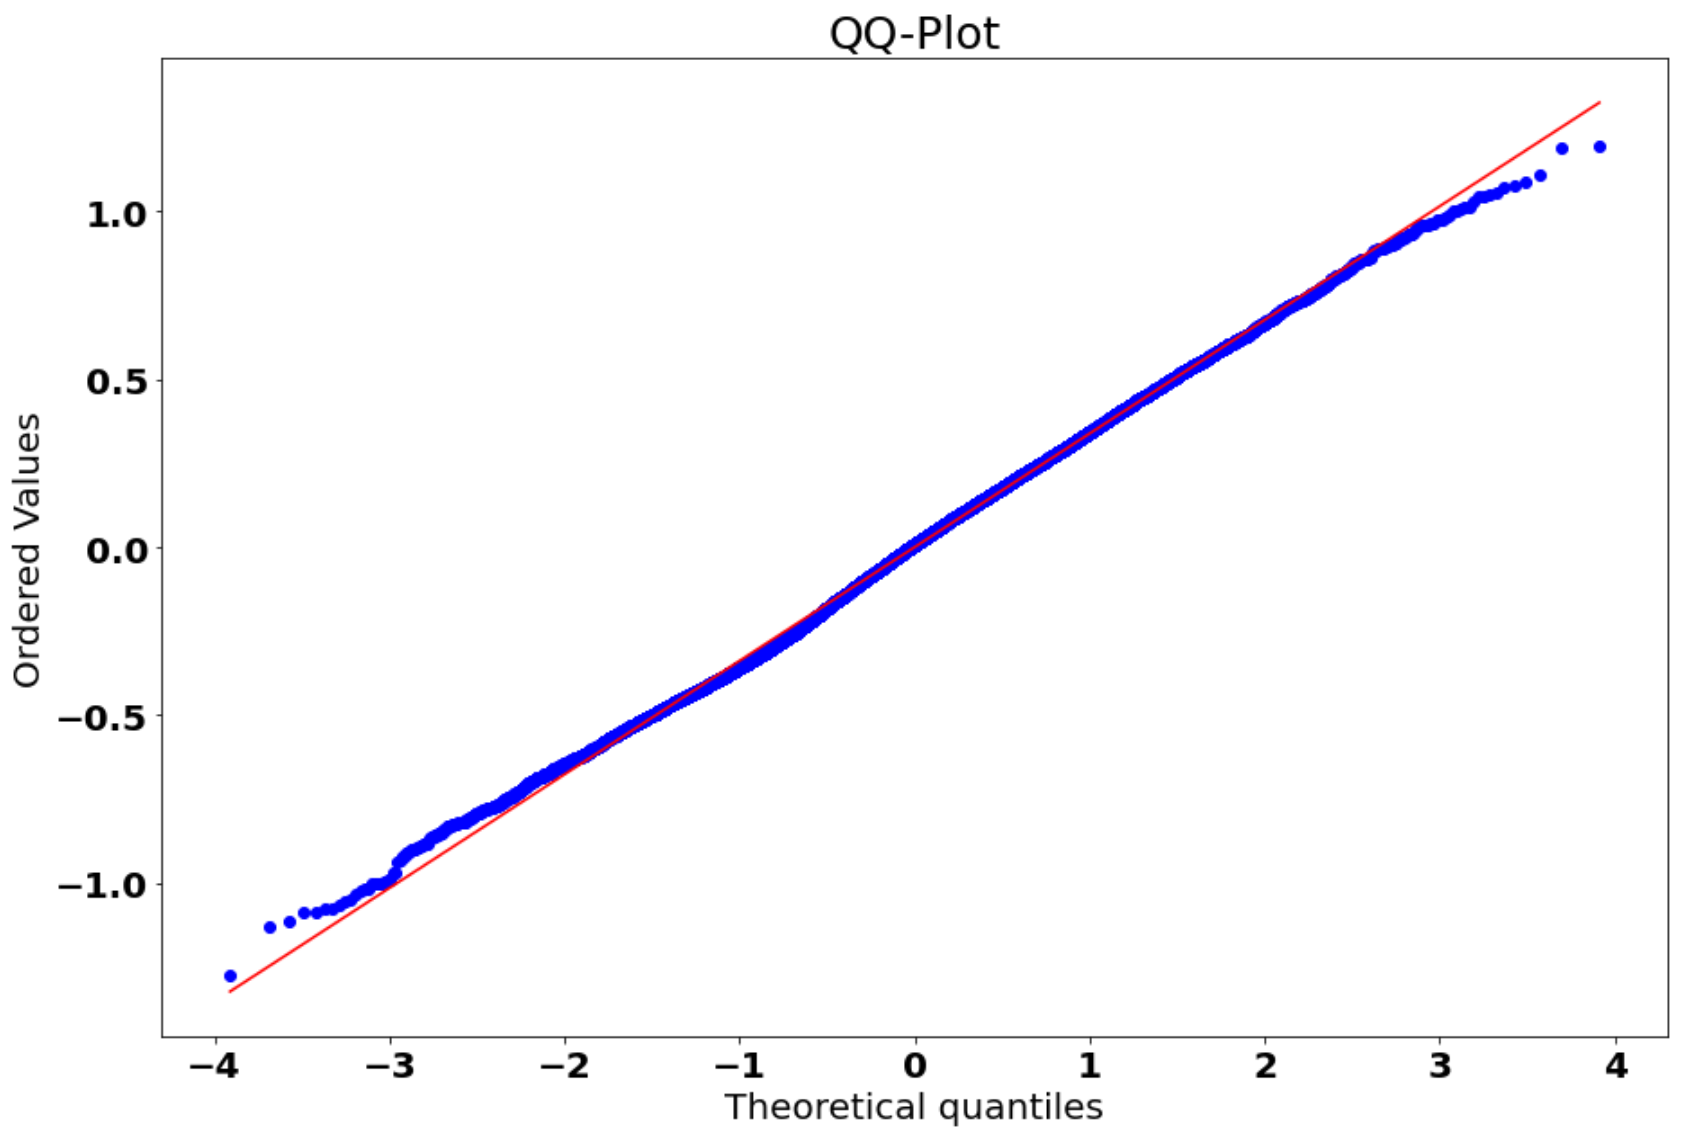
\includegraphics[width=3in,height=2in]{qq_plot_multi_model}
	\end{center}%
}
\frame{
\frametitle{Normality Assumption for Errors 2}
\begin{center}
	\textbf{DISTRIBUTIONS PLOT OF RESIDUALS}\\
	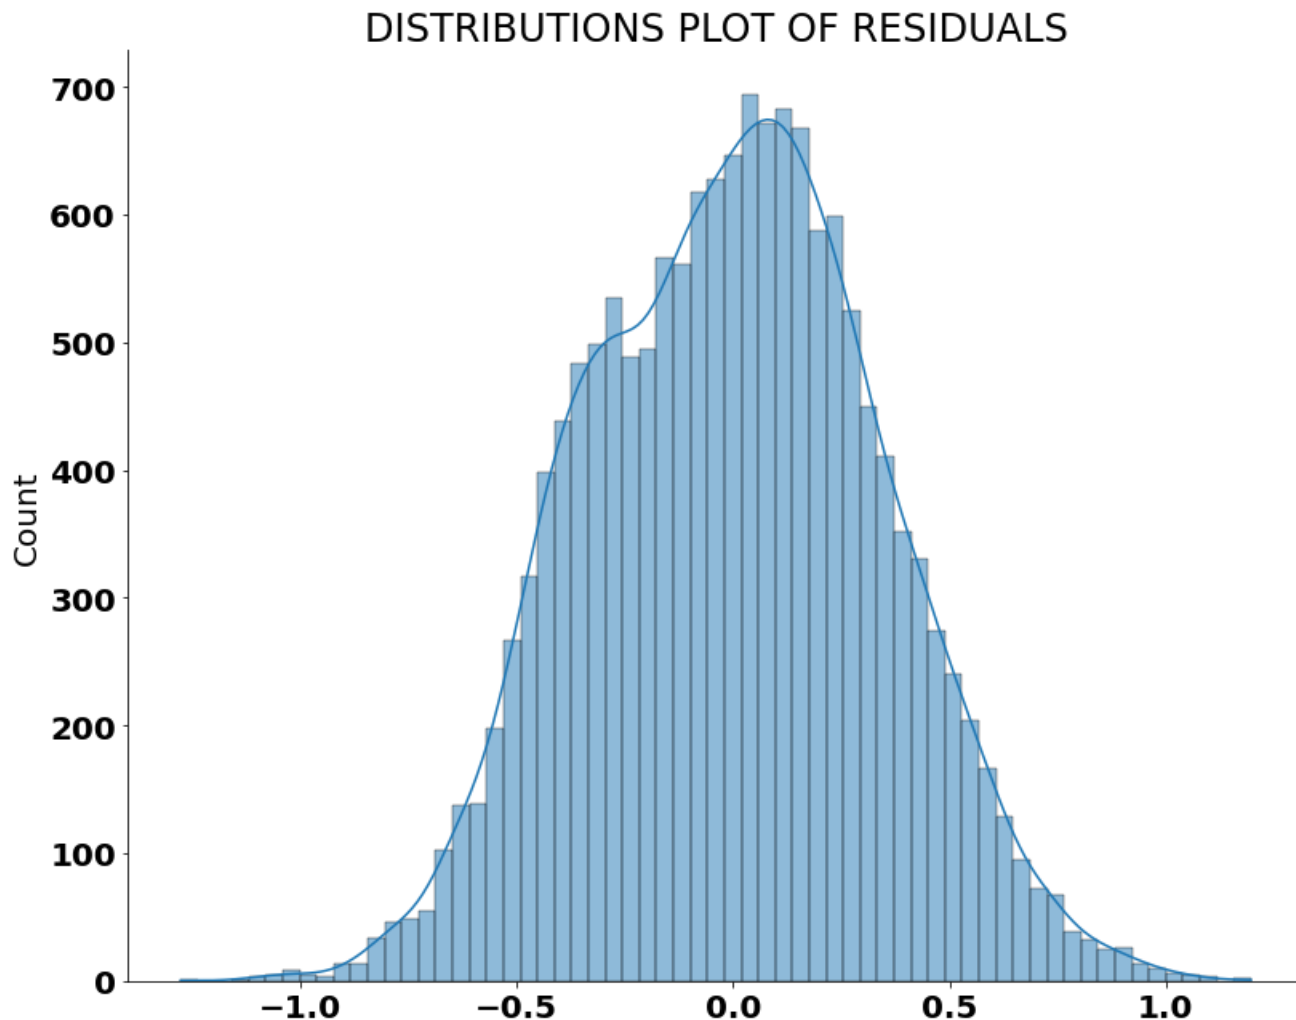
\includegraphics[width=3in,height=2in]{dist_plot_resid_multi_model}
\end{center}%
}
\frame{
\frametitle{Normality Assumption for Errors 3}
I also, used D'Agostino Test for Normality:\\
\textbf{The Null Hypothesis:} \\
The Residuals are normally distributed,\\
\textbf{The Alternative Hypothesis:}\\  The Residuals are not normally distributed.
\vskip 0.2in
\begin{itemize}
	\item Our p-value for this model is \(p=0.000 < 0.05 = \alpha\).
	\item We have enough evidence to reject the Null Hypothesis 
	\item We conclude that D'Agostino Test tells us, that residuals are not normally distributed.
\end{itemize}
}
\frame{
\frametitle{Normality Assumption for Errors 4}
\textbf{Conclusion for Normality:}
\pause
\vskip 0.3in
\begin{itemize}
	\item  Based on QQ-Plot, Distributions Plot, and D'Agostino Test, I conclude that the Distribution of Errors is not far away from Normal.
	\vskip 0.3in
	\item  Also, since we have a lot of observations Normality Assumption doesn't play a critical role, since Central Limit Theorem will apply in this case.
\end{itemize}
}
\frame{
\frametitle{Constant Error Variance 1}
To check if heteroscedasticity is present in the model, I used Residual-vs-Predicted values plot and Breusch-Pagan test.
I look at at the Residual-vs-Predicted values plot first.
\begin{center}
	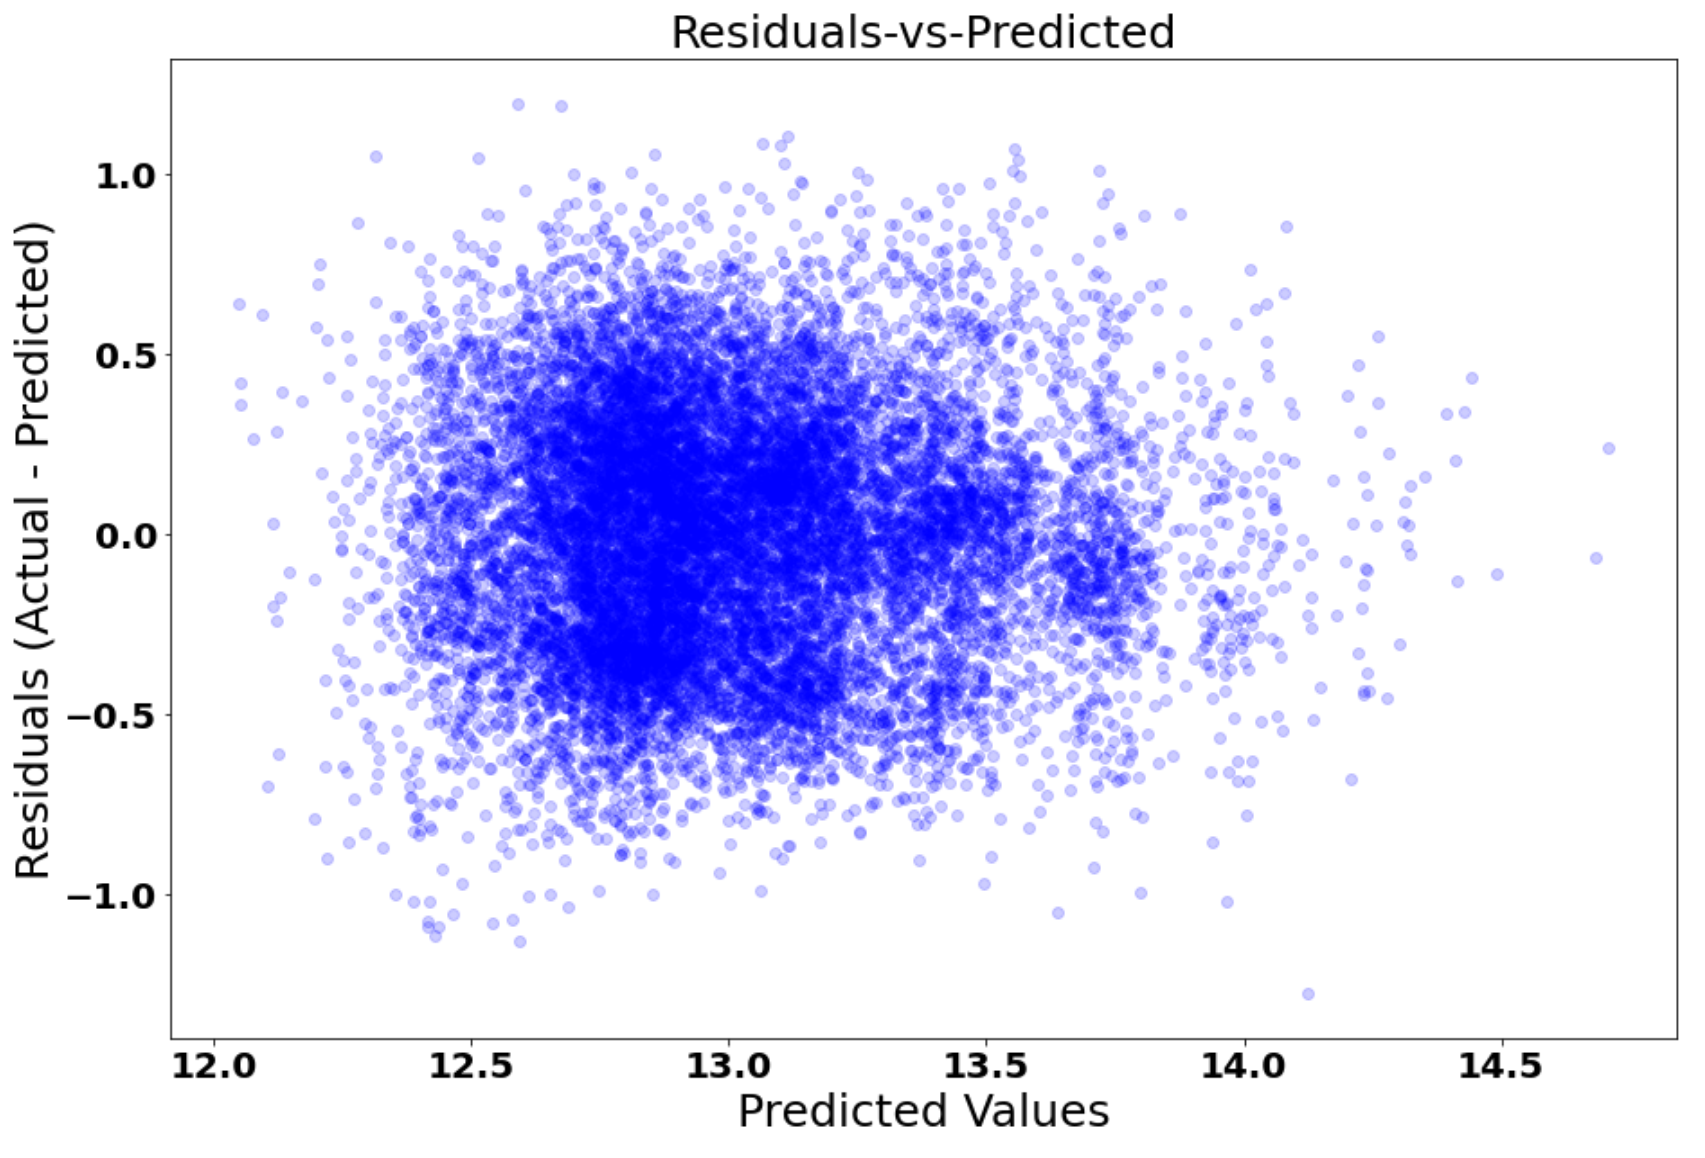
\includegraphics[width=3in]{residual_plot_multi_model}
\end{center}
}
\frame{
\frametitle{Constant Error Variance 2}
I used Breusch-Pagan Test:\\
\textbf{The Null Hypothesis:}\\ 
 Homoscedasticity is present.\\
\textbf{The Alternative Hypothesis:}  Homoscedasticity is not present (i.e. heteroscedasticity exists).\\
\vskip 0.3in
\pause
\begin{itemize}
	\item Our p-value for this model is \(p=0.000 < 05 = \alpha\).  
	\item We  have enough evidence to reject the Null Hypothesis.
	 \item We conclude from Breusch-Pagan Test, that we have don't have heteroscedasticity.\\
\end{itemize}
}
\frame{
\frametitle{Constant Error Variance : Conclusion} 
\begin{center}
	From the Residual-vs-Predicted values plot and  Breusch-Pagan Test, I conclude that we  have some Heteroscedasticity in our model, but it is not very bad.
\end{center}
}
\frame{
	\frametitle{Overall Conclusion:}
	\begin{center}
		\textbf{ I conclude that our model almost satisfies statistical assumptions for the regression model.}
	\end{center}
}
\subsection{Explanation of the Model}
\frame{
\frametitle{Model}
\begin{align*}
	\ln(price) =& 10.2082 + 0.3618\cdot \text{waterfront} - 0.0160\cdot\text{bedrooms} \\-&
	0.0153 \cdot\text{bathrooms}  + 0.1400\cdot\text{sqft\_living}^{0.3} + 0.0088 \cdot \text{floors}\\
	+& 0.1494\cdot\text{view}^{0.5}+ 0.0105\cdot\text{grade}^2+0.1187\cdot\ln\left(\text{sqft\_living15}\right)
\end{align*}
}
\frame{
\frametitle{Explanation of the Model}
Before I begin explain the coefficients, I notice that $P>|t|$ for the {\it floors} variable is $0.155$, which makes  {\it floors} insignificant for the analysis. 
}
\frame{
\frametitle{Intercept}
\begin{itemize}
	\item  The model has the sample intercept of $10.2082$.
	\vskip 0.3in 
	\pause
	\item If we assume that all explanatory variables are zeros, this would mean that the price would be $e^{10.2082}\approx 27,124$
\end{itemize}
}
\frame{
\frametitle{$0.3618$ is the coefficient for {\it waterfront}}
\begin{itemize}
	\item {\it Waterfront} is a categorical variable coded as $0$ or $1$, a one unit difference represents switching from one category to the other. $10.2082$ is then the average difference in  {\it price} between the category for which  {\it waterfront} = \(0\) (no waterfront) and the category for which  {\it waterfront} = \(1\) (the house has a waterfront). 
	\vskip 0.2in
	\pause
	So compared to $\ln(\text{\it price})$ of the house with no waterfront, we would expect the $\ln(\text{\it price})$ for the house with waterfront to be $0.3618$ higher, on average, if we fix all other explanatory variables.
\end{itemize}
}
\frame{
	\frametitle{$0.3618$ is the coefficient for {\it waterfront}}
Let $y_2 = \text{price of the house with waterfront}$   and $y_1 = \text{price of the house with no waterfront}$, then 
$$
\large
\ln y_2 - \ln y_1 = 0.3618 \implies \ln \frac{y_2}{y_1} = 0.3618 \implies \frac{y_2}{y_1} = e^{0.3618}$$
To understand the change in {\it price} in percents, if we switch from the house with no waterfront to the house with waterfront while keeping all other variables the same, will use the following formula:
$$
\large
100\times \left[\frac{y_2-y_1}{y_1}\right]= 100\times \left[\frac{y_2}{y_1} - 1\right] = 100\times \left[ e^{0.3618} - 1\right] \approx 43.59\%$$
}
\frame{
	\frametitle{$0.3618$ is the coefficient for {\it waterfront}}	
Switching from the house with no waterfront to the house with waterfront while keeping all other explanatory variables fixed, will increase the price by 43.59\%.
}
\frame{
\frametitle{$-0.0160$ is the coefficient for number of {\it bedrooms}}
Let $y_2 = \text{price}$ for the house with $x_2$ number of bedrooms and $y_1 = \text{price}$ for the house with $x_1$ number of bedrooms, then 
\begin{align*}
	\ln y_2 - \ln y_1 =& -0.016 x_2 - (-0.016 x_1) \\
	=& -0.016 (x_2 - x_1) \implies \ln\frac{y_2}{y_1} = -0.016 (x_2-x_1)\\
	\implies& \frac{y_2}{y_1} = e^{-0.016(x_2-x_1)}
\end{align*}
}
\frame{
\frametitle{$-0.0160$ is the coefficient for number of {\it bedrooms}}
If we increase the number of bedrooms by 1 while keeping the other variables fixed and use percents, we will get the following
$$
\large
100 \times \left[\frac{y_2}{y_1} - 1 \right] = 100 \times \left[e^{-0.016} -1 \right] \approx -1.58\%
$$
\begin{itemize}
	\item Thus, increasing the number of bedrooms by 1 while keeping the other variables fixed, will decrease the price of the house by 1.58\%. 
\end{itemize}
}
\frame{
\frametitle{$-0.0153$ is the coefficient for number of {\it bathrooms}}
\begin{enumerate}
	\item  The same explanation we have for $-0.0153$ which a coefficient for number of bathrooms.
	\vskip 0.3in
	\pause
	\item  If we increase the number of bathrooms by 1 while keeping the other variables fixed, will decrease the price of the house by 1.51\%. 
\end{enumerate}
}
\frame{
\frametitle{$0.1400$ is the coefficient for {\it sqft\_living}}
Let $y_2 = \text{price}$ for the house with $x_2$ {\it sqft\_living} and $y_1 = \text{price}$ for the house with $x_1 =$ {\it sqft\_living}, then 
\begin{align*}
\ln y_2 - \ln y_1 = &0.1400 x_2^{0.3} - 0.1400 x_1^{0.3} \implies \ln \frac{y_2}{y_1} = 0.1400 \left( x_2^{0.3} - x_1^{0.3}\right) \\
& \implies \frac{y_2}{y_1}=e^{0.1400 \left( x_2^{0.3} - x_1^{0.3}\right)}
\end{align*}
If we increase the {\it sqft\_living} from $1000ft$ to $1100ft$ while keeping the other variables fixed, we will get the following change in price in percents:
$$
100 \times \left[\frac{y_2}{y_1} -1  \right] = 100 \times \left[ e^{0.1400 \left( 1100^{0.3} - 1000^{0.3}\right)} - 1 \right]\approx 3.28\%
$$
}
\frame{
\frametitle{$0.1400$ is the coefficient for {\it sqft\_living}}
\begin{itemize}
	\item If the {\it sqft\_living} is $1000ft$ and we increase it to $1100ft$ while keeping the other variables fixed, we will get the change in price of $3.28\%$.
	\vskip 0.3in
	\pause
	\item In this particular example $10\%$ change in {\it sqft\_living} starting from $x_1 = 1000ft$ forces $3.28\%$ change in price.
\end{itemize}
}
\frame{
	\frametitle{$0.1494$ is the coefficient for the {\it view}}
	The coefficient for the {\it view} has the same explanation as the {\it sqft\_living}. 
	\vskip 0.3in
	\pause
	If we increase the {\it view} by $1$ unit from $2$ to $3$ while keeping the other variables fixed, we will get the following:
	$$
	\large 
	100 \times \left[\frac{y_2}{y_1} -1  \right] = 100 \times \left[ e^{0.1494 \left( 3^{0.5} - 2^{0.5}\right)} - 1 \right]\approx 4.86\%
	$$
	In this particular example if the {\it view} will increase from $2$ to $3$, the price will increase by 4.86\%.
}
\frame{
\frametitle{$0.0105$ is the coefficient for the {\it grade}}
 The coefficient for the {\it grade} has the same explanation as the {\it sqft\_living}.
 \vskip 0.3in
 \pause
  If we increase the {\it grade} by $1$ unit from $2$ to $3$ while keeping the other variables fixed, we will get the following:
$$
\large 
100 \times \left[\frac{y_2}{y_1} -1  \right] = 100 \times \left[ e^{0.0105\left( 3^{2} - 2^{2}\right)} - 1 \right]\approx 5.39\%
$$
In this particular example if the {\it grade} will increase from $2$ to $3$ while other variables stay the same, the price will increase by 5.39\%.
}
\frame{
\frametitle{$0.1187$ is the coefficient for the {\it sqft\_living15}}
 Let $y_2 = \text{price}$ for the house with $x_2$ {\it sqft\_living15} and $y_1 = \text{price}$ for the house with $x_1$ {\it sqft\_living15}, then 
\begin{align*}
\ln y_2 - \ln y_1 = & 0.1187 \ln x_2 - 0.1187 \ln x_1 \implies \ln \frac{y_2}{y_1} = 0.1187 \ln \frac{x_2}{x_1}\\  \implies & \frac{y_2}{y_1} = \left(\frac{x_2}{x_1}\right)^{0.1187}
\end{align*}
The change in price in percent will be:
$$
100 \times \left[\frac{y_2}{y_1} - 1 \right]= 100 \times \left[ \left(\frac{x_2}{x_1}\right)^{0.1187} - 1 \right]
$$
}
\frame{
\frametitle{$0.1187$ is the coefficient for the {\it sqft\_living15}}
In this particular example, if we increase the {\it sqft\_living15} by $100$ units from $1000$ to $1100$ while keeping the other variables fixed, we will get the following:
$$
100 \times \left[ e^{0.1187}\times \frac{1100}{1000} - 1 \right] \approx 1.14\%
$$
Thus, 10\% increase in {\it sqft\_living15} will lead to 1.14\% increase in {\it price}.
}
\frame{
	\frametitle{\(R^2\)}
	\begin{itemize}
		\item The model has \(R^2\approx 0.5\).  
		\vskip 0.3in
		\pause
		\item This means that our model explains about 50\% of the variation by using {\it sqft\_living} as independent variable.
	\end{itemize}
}
\frame{
\frametitle{ANOVA}
Is our model with many explanatory variable better than the model with zero explanatory variables?\\
Our model has \(F-statistic = 1.737\times 10^4\)  and \(Prob > F\) is \(0.000\).
\vskip0.3in
\pause
\textbf{The Null Hypothesis:}   The slope\(=0\)\\
\vskip 0.3in
\pause
\textbf{The Alternative Hypothesis:} The slope\(\ne 0\)
}
\frame{
\frametitle{ANOVA}
\begin{itemize}
	\item Our p-value for this model is \(p=0.000 < 0.05 = \alpha\). 
	\item We have enough evidence to reject the Null Hypothesis at $5\%$ level of significance
	 \item We conclude that the Test  tells us, that at least one of the coefficients is not $0$. 
	 \item Since our p-value is $0$, there is a $0\%$ probability that the improvements that we are seeing with our independent variables model are due to random chance alone.
\end{itemize}
}
\section{Conclusions}
\subsection{Data Modeling}
\begin{frame}
	\frametitle{Conclusions: Data Modeling}
	 I used the following steps during data modeling:
	\begin{itemize}
		\item  Dropped 2376 rows where {\it waterfront} is NaN.
		\item  Dropped 63 rows where {\it view} is NaN.
		\item Dropped 3842 rows where {\it yr\_renovated} is NaN.
		\item I converted {\it sqft\_basement}  string format into float.
		\item  During modeling dropped outliers when necessary.
	\end{itemize}
\end{frame}
\subsection{Modeling}
\frame{
\frametitle{Conclusions: Modeling}
\begin{itemize}
	\item I built two models:
	\begin{itemize}
		\item  Linear Regression Model
		\item Multiple Linear Regression Model
	\end{itemize}
	\item  I checked whether the models satisfy statistical assumptions of Linear Regression
	\item  I explained the models.
	\item Models can be used for interpolation given the data about a particular property.
\end{itemize}
}
\subsection{Ways to improve the analysis}
\frame{
\frametitle{Conclusions: Ways to Improve the Analysis}
\begin{itemize}
	\item More data wrangling is need to remove {\it heteroscedasticity} from the Multiple Linear Regression Model.
	\item  Include more explanatory variables.
	\item Scrape webpages for more data such as school grade, crime rate, etc. for properties.
\end{itemize}
}
\frame{
\begin{center}
	\LARGE
	THE END \\
	THANK YOU!
\end{center}
}
\end{document}